\chapter{Theoretical Framework} \label{cap:theoretical}

% 3. Wireless Sensor Networks (WSN) and Communication Technologies
% Focus on how WSN enables data collection, data transmission, and real-time monitoring.
% Discussion on technologies like LoRa, LPWAN, Zigbee, bt, web.
% LoRa and LPWAN dominance in environmental WSN
% Architectures? Mesh vs. star topologies. Use of gateways, cloud services, and edge computing nodes etc

% Relevant Articles:
% "Long Battery Life IoT Sensing by Beat Sensors" — Communication based on timing intervals. (Observation: Alternative low-power communication model.)
% "Exploiting hardware vulnerabilities to attack embedded system devices" — Security challenges in WSN. (Observation: Survey of microarchitectural attacks.)
% "Conception and Design of WSN Sensor Nodes Based on Soil Moisture Monitoring" — Also relevant here for its WSN node design discussion.

% "LoRa provided reliable communication over 5km in rural tests."
% "Battery life extended to 5 years using beat sensors."
% Mention the use of AI/ML for sensor data analysis, anomaly detection, or pattern recognition. Some articles on water monitoring use CNN-based object detection for water level estimation.


This chapter presents the theoretical foundation underpinning the development of the proposed water level monitoring system. It discusses the essential technologies and concepts, including the \glsxtrfull{IoT}, long-range wireless communication (\glsxtrfull{LoRa}/\gls{LoRaWAN}), distance measurement methods such as \glsxtrfull{LiDAR} and ultrasonic sensors, and embedded systems. These topics establish the context and technical justification for the architecture adopted in this work.

\section{IoT}

The \gls{IoT} encompasses a network of interconnected physical objects that are equipped with sensors, processors, and communication interfaces, allowing them to collect, process, and transmit data without human intervention . The proliferation of \gls{IoT} has enabled the deployment of intelligent systems in areas such as agriculture, industrial monitoring, and environmental surveillance. \cite{Madakam:2015,javaid_2021_sensors}

In this project, \gls{IoT} concepts are applied to create an autonomous and distributed sensor network capable of collecting hydrological data and transmitting it remotely for analysis and visualization. The figure \ref{fig:iot} illustrates how various devices connect to the internet through \gls{IoT}, enabling data exchange and interaction between the physical and digital worlds. \cite{javaid_2021_sensors}

\begin{figure}[h]
    \centering
    \caption{Internet of Things.}
    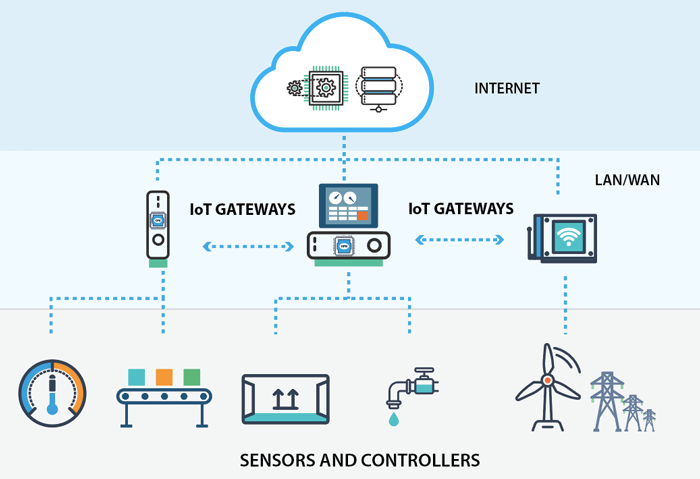
\includegraphics[width=0.8\textwidth]{figuras/iot.png}
    \fonte{\cite{iot123}.}
    \label{fig:iot}
\end{figure}

\section{LoRa and LoRaWAN}

\glsxtrfull{LoRa} is a proprietary spread spectrum modulation technique on the basis of \glsxtrfull{CSS}, which is resilient and robust against interference and noise, it also provides a solution for long-range and ultra-low power-consumption transmission, using unlicensed radio bands such as 868 MHz (Europe) and 915 MHz (Americas) \cite{sun_2022_recent}.

\glsxtrfull{LoRaWAN} is the \glsxtrfull{MAC} protocol built on top of \gls{LoRa}, specifying how end-devices communicate with central gateways and application servers,  defining a typical star-topology network architecture and its bi-directional communication protocol. The technology has been designed for applications that need to send small amounts of data over long distances a few times per day. Its low power features offers the capability to achieve autonomy of up to 10 years. \cite{pule_2017_wireless,sun_2022_recent}. Such long-range and energy-efficient communication demands have inspired the emergence of Low Power Wide Area Networks (LPWANs) as a new \gls{IoT} paradigm, which fills the gap of legacy wireless communication technologies shown in Figure \ref{fig:lora}. 

\begin{figure}[h]
    \centering
    \caption{Comparison with legacy wireless communication technologies.}
    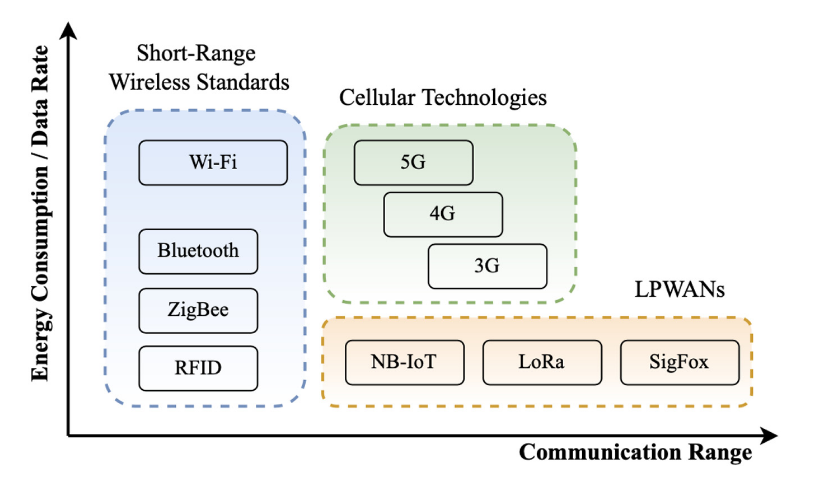
\includegraphics[width=0.8\textwidth]{figuras/Lora-comparison.png}
    \fonte{\cite{sun_2022_recent}.}
    \label{fig:lora}
\end{figure}

\section{Microcontroller ESP8266}

Embedded systems are specialized computing systems designed to perform dedicated functions within larger systems, often under real-time constraints. The NodeMCU ESP8266 is a microcontroller based on the ESP8266 platform, which features integrated Wi-Fi connectivity. It is widely used in \gls{IoT} projects due to its ease of programming, low cost, and advanced features. The ESP8266, shown in Figure \ref{fig:node}, is particularly suitable for such applications due to its ability to operate at low power, which is crucial for battery-powered devices, and its capability to connect to Wi-Fi networks, enabling communication with the internet and other devices on the network \cite{Kolban2016}.\cite{datasheet_2023_esp8266ex}

\begin{figure}[h]
    \centering
    \caption{ESP8266 NodeMcu.}
    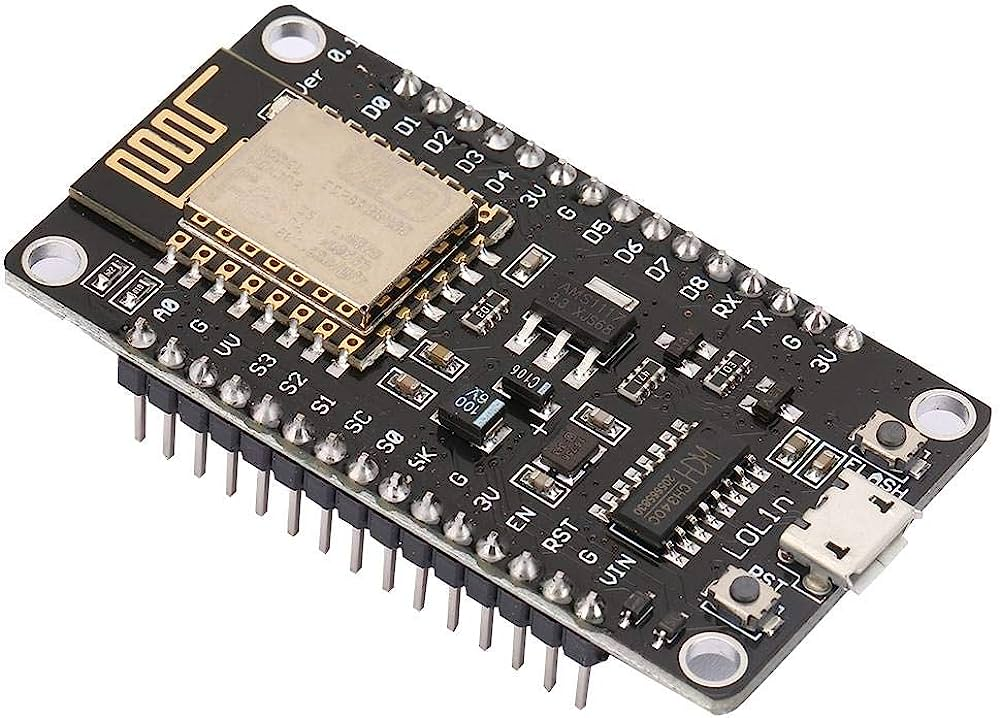
\includegraphics[width=0.5\textwidth]{figuras/nodemcu.jpg}
    \fonte{\cite{nodemcu}.}
    \label{fig:node}
\end{figure}

\section{LiDAR}

\glsxtrfull{LiDAR} technology enables the accurate determination of an object's distance (and velocity) information. LiDAR technology is widely used in metrology, environment monitoring, archaeology, and robotics. Compared with more mature \glsxtrfull{RADAR} technology, LiDAR makes use of optical wave, which is at shorter wavelength regime compared with radio wave, and hence has potential to achieve higher precision in 3D sensing.\cite{li_2022_a, lednev_2013_remote,behroozpour_2017_lidar,javaid_2021_sensors}.

The principle of lidar ranging relies on the rugosity of the reflective surface to generate nonspecular reflection (i.e., scattering) of the incipient laser beam. As with radar, lidar ranging measures time of flight, but it uses higher frequency waves for greater pulse intensities. Near-infrared (NIR) light is most commonly used for this purpose, typically over wavelengths of 900–1,100 nm (270–330 THz) due to the low cost of lasers operating in this wavelength range and lower energy density than the visible spectrum.\cite{li_2022_a, fernandezdiaz_2014_early, smart_2009_river, behroozpour_2017_lidar}. The laser wavelength is a critical factor in determining the sensor's performance, as it influences the interaction with water and suspended particles. Figure \ref{fig:laser-wavelength-graphs} illustrates the spectral character of clear still water as a function of laser wavelength and the influence of suspended sediment concentration on reflectance in rivers \cite{lednev_2013_remote,milan_2010_mapping,paul_2020_a}.

\begin{figure}[h]
    \centering
    \caption{(a) Spectral character of clear still water as a function of laser wavelength \cite{lednev_2013_remote,milan_2010_mapping}. (b) Influence of suspended sediment concentration (curves: units of mg L(-1)) in river upon reflectance \cite{paul_2020_a, milan_2010_mapping}}
    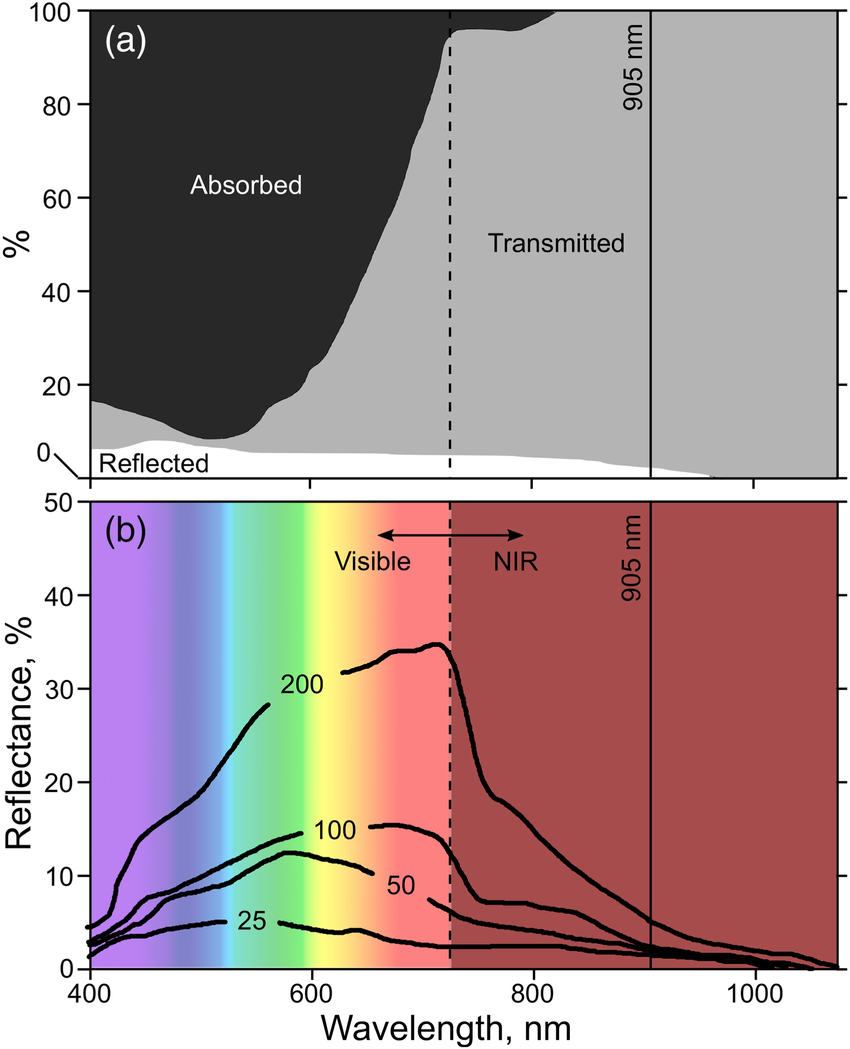
\includegraphics[width=0.8\textwidth]{figuras/light-absorption.png}
    \fonte{\cite{lednev_2013_remote,milan_2010_mapping,paul_2020_a}.}
    \label{fig:laser-wavelength-graphs}
\end{figure}

The three sensing schemes most commonly used in LiDAR sensors are: pulsed \glsxtrfull{TOF}, AMCW \gls{TOF}, and FMCW. \cite{li_2022_a,behroozpour_2017_lidar}. For this work the most important ones are the pulsed \gls{TOF} and AMCW \gls{TOF}, which are described below.

\subsection{Pulsed Time of Flight (TOF)}
The pulsed TOF LiDAR works based on the time delay of an optical pulse emitted by the TX, reflected from the sensing object, and received by the RX. The sensing distance can be expressed using the following equation \cite{li_2022_a}.

\begin{equation}
    d = \frac{c \cdot \Delta t}{2}
\end{equation}

where \(d\) is the distance to the object in meters, \(c\) is the speed of light, and \( \Delta t\) is the time delay between emission and reception of the optical pulse in seconds.

\subsection{Amplitude Modulated Continuous Wave (AMCW) Time of Flight (TOF)}
AMCW TOF LiDAR uses a continuous wave laser that is modulated in amplitude. The phase difference between the transmitted and received signals is measured to determine the distance to the object. The distance can be calculated using the following equation \cite{li_2022_a}.

\begin{equation}
    d = \frac{c \cdot \Delta \phi}{4\pi f}
\end{equation}

where \(d\) is the distance to the object in meters, \(c\) is the speed of light, \(\Delta \phi\) is the phase difference between the transmitted and received signals, and \(f\) is the modulation frequency in Hz.

\section{Ultrasonic Sensors}

Ultrasonic sensors estimate distance by transmitting high-frequency acoustic waves and measuring the echo delay. Common models like the HC-SR04 and JSN-SR04T are widely used in academic and industrial applications due to their low cost and simplicity \cite{bresnahan_2023_a,akhileshnagpure_2022_water,mohammadrezamasoudimoghaddam_2024_a}.

The basic principle of ultrasonic distance measurement is based on the time of flight (\gls{TOF}) of sound waves. The sensor emits a high-frequency sound wave, which travels through the air, reflects off an object, and returns to the sensor.

\section{Wireless Sensor Network (WSN)}

\glsxtrfull{WSN} are considered a promising alternative to complement conventional monitoring processes. These networks are relatively affordable and allow measurements to be taken remotely, in real-time and with minimal human intervention \cite{pule_2017_wireless}. A \gls{WSN} is composed of spatially distributed autonomous nodes that monitor physical or environmental conditions. These nodes typically consist of a sensing unit, processing unit, communication interface, and power source. Natural disaster monitoring is very complex and imposes a number of challenges mainly due to huge scales,uncertainties, and harsh environments.

Each such sensor network node typically has many parts: a radio transceiver with an internal antenna or connection to an external antenna, a microcontroller, an electronic circuit for interfacing with the sensors and an energy source, usually a battery or an embedded form of energy harvesting \cite{yellampalli_2021_wireless}. An example architecture of a WSN is shown in Figure \ref{fig:wsn-graphs}. The nodes are capable of collecting data from the environment, processing it, and transmitting it wirelessly to a base station or gateway for further analysis and visualization. A \gls{WSN} can be single hop, where the nodes connect directly to the base station, or multi-hop, where the nodes can send information between themselves before reaching the base station \cite{yellampalli_2021_wireless}.

\begin{figure}[h]
    \centering
    \caption{Wireless Sensor Network architecture.}
    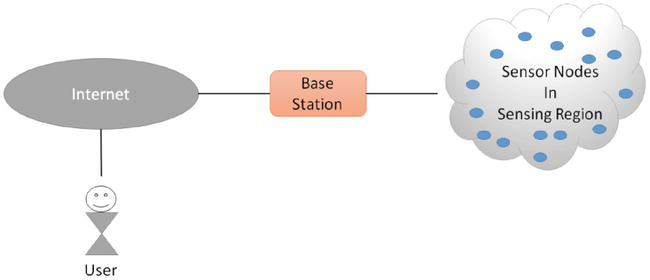
\includegraphics[width=0.8\textwidth]{figuras/WSN_architecture.png}
    \fonte{\cite{yellampalli_2021_wireless}.}
    \label{fig:wsn-graphs}
\end{figure}

WSN-based natural disaster monitoring systems excel in terms of cost, speed of response, scalability and flexibility in contrast to conventional approaches. In general, disaster monitoring with WSN manifests a typical paradigm of data-intensive application upon low-cost scalable system \cite{chen_2013_natural, pule_2017_wireless, ferreira_2023_conception}. In this work, the \gls{WSN} architecture facilitates distributed hydrological data collection and centralized data aggregation through \gls{LoRa} communication.

\section{Time-Series Data and Environmental Monitoring}

Time-series data represent sequential observations over time. In the context of water level monitoring, time-series analysis enables the detection of trends, anomalies, and correlations between environmental factors \cite{lozano_2017_sensors}. Basic statistical techniques—such as moving averages, root mean square error (\glsxtrfull{RMSE}), and filtering—are applied to improve data reliability and reduce noise\cite{santana_2024_development}. 

